\documentclass[border=1mm]{standalone}
\usepackage[T1]{fontenc}
\usepackage[scaled=0.92]{helvet}
\renewcommand\familydefault{\sfdefault}
\usepackage{amssymb}
\usepackage{tikz}
\usetikzlibrary{arrows.meta,calc,shapes.geometric}
% ---- shared style (methodology figures) ----
\definecolor{mA}{HTML}{1B7F79}\definecolor{mAl}{HTML}{E4F2F0}
\definecolor{mB}{HTML}{2F5F98}\definecolor{mBl}{HTML}{E7EEF7}
\definecolor{mC}{HTML}{B85A16}\definecolor{mCl}{HTML}{FBEEDF}
\definecolor{ink}{HTML}{262626}\definecolor{mute}{HTML}{6B6B6B}
\definecolor{grey}{HTML}{8C8C8C}\definecolor{greyl}{HTML}{EFEFEF}
% pathway colours: ECM, TGF-beta, stellate, inflammation, apoptosis/stress, hepatocyte
\definecolor{pw0}{HTML}{B85A16}\definecolor{pw1}{HTML}{D9A21B}\definecolor{pw2}{HTML}{8A5BA6}
\definecolor{pw3}{HTML}{C2413B}\definecolor{pw4}{HTML}{6E8B3D}\definecolor{pw5}{HTML}{2F5F98}
\newcommand\fs{\fontsize{7}{8.4}\selectfont}
\newcommand\fss{\fontsize{6.3}{7.5}\selectfont}
\newcommand\fsx{\fontsize{5.8}{6.8}\selectfont}
\newcommand\fsh{\fontsize{7.6}{9}\selectfont\bfseries}
\newcommand\fsn{\fontsize{9}{10}\selectfont\bfseries}
\hyphenpenalty=10000 \exhyphenpenalty=10000
\tikzset{
  >={Stealth[length=2mm,width=1.6mm]},
  flow/.style={->,line width=0.8pt,draw=ink!70},
  thin/.style={->,line width=0.5pt,draw=ink!60},
  gedge/.style={draw=black!22,line width=0.25pt},
  gnode/.style={circle,draw=white,line width=0.25pt,inner sep=0pt,minimum size=1.45mm},
  ttl/.style={anchor=west,font=\fsh},
}
% cylinder: \cyl{colour}{x centre}{base y}{height}{width}
\newcommand\cyl[5]{%
  \filldraw[fill=#1!35,draw=#1,line width=0.5pt] ({#2-#5/2},{#3+#4}) -- ({#2-#5/2},#3) arc[start angle=180,end angle=360,x radius=#5/2,y radius=0.9] -- ({#2+#5/2},{#3+#4});
  \filldraw[fill=#1!12,draw=#1,line width=0.5pt] (#2,{#3+#4}) ellipse[x radius=#5/2,y radius=0.9];}
% numbered module badge
\newcommand\badge[3]{\node[circle,fill=#1,text=white,inner sep=0pt,minimum size=4.6mm,font=\fss\bfseries] at #2 {#3};}
\newcommand\lk[1]{\node[diamond,fill=mC,inner sep=0pt,minimum size=1.9mm] at #1 {};}
% mini graph: \mg{cx}{cy}{scale}{edge list}{c1,...,c6}
\newcommand\mg[5]{\begin{scope}[shift={(#1,#2)},scale=#3]
  \coordinate (q1) at (0,1.7); \coordinate (q2) at (1.6,0.6); \coordinate (q3) at (1.0,-1.3);
  \coordinate (q4) at (-1.0,-1.3); \coordinate (q5) at (-1.6,0.6); \coordinate (q6) at (0,0);
  \edef\elist{#4}\edef\clist{#5}\foreach \a/\b in \elist \draw[ink!45,line width=0.45pt] (q\a)--(q\b);
  \foreach \c [count=\k] in \clist \node[circle,fill=\c,draw=white,line width=0.3pt,inner sep=0pt,minimum size=1.7mm] at (q\k) {};
\end{scope}}
\def\Est{1/2,1/5,2/6,5/6,6/3,6/4,3/4}
\def\Cst{pw0,pw0,pw1,pw2,pw5,pw3}
% test tile: \tile{x}{id}{name}{caption}{negative if}
\newcommand\tile[5]{%
  \fill[white,rounded corners=1.2mm] (#1,14) rectangle ++(24.8,56);
  \draw[mC!70,line width=0.5pt,rounded corners=1.2mm] (#1,14) rectangle ++(24.8,56);
  \fill[mC,rounded corners=1.2mm] (#1,70) rectangle ++(24.8,-8.4);
  \fill[mC] (#1,61.6) rectangle ++(24.8,1.5);
  \node[circle,fill=white,text=mC,inner sep=0pt,minimum size=4.2mm,font=\fss\bfseries] at (#1+3,65.8) {#2};
  \node[anchor=west,text=white,font=\fss\bfseries,text width=18mm,align=left] at (#1+5.6,65.8) {#3};
  \node[font=\fsx,text=mute,text width=23mm,align=center] at (#1+12.4,32.4) {#4};
  \fill[mCl,rounded corners=0.9mm] (#1+1,15) rectangle ++(22.8,10.6);
  \node[font=\fsx\bfseries,text=mC] at (#1+12.4,22.6) {negative if};
  \node[font=\fss\bfseries,text=ink] at (#1+12.4,18.4) {#5};}
\begin{document}
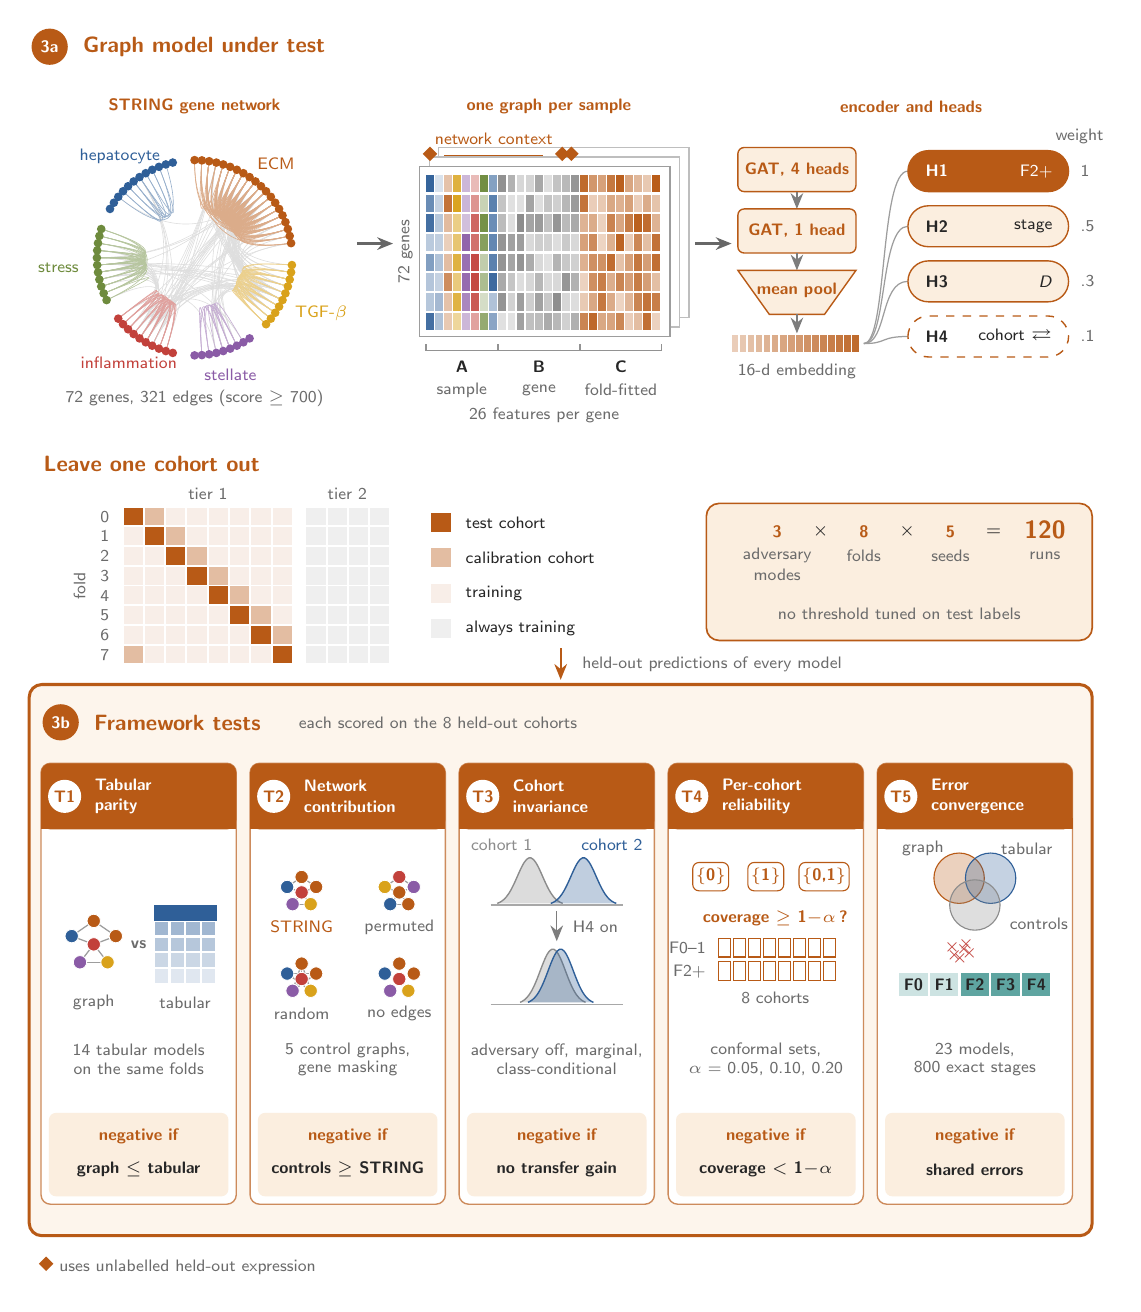
\begin{tikzpicture}[x=1mm,y=1mm,font=\fs,text=ink]
% =================== 3a: graph model ===================
\badge{mC}{(2.6,161)}{3a}
\node[ttl,text=mC] at (5.6,161) {Graph model under test};
% ---- real STRING graph ----
\node[font=\fss\bfseries,text=mC] at (21,153.4) {STRING gene network};
\coordinate (O) at (21.0,134.2);
\foreach \i/\a in {0/90.0,1/85.7,2/81.4,3/77.1,4/72.9,5/68.6,6/64.3,7/60.0,8/55.7,9/51.4,10/47.1,11/42.9,12/38.6,13/34.3,14/30.0,15/25.7,16/21.4,17/17.1,18/12.9,19/8.6,20/-4.3,21/-8.6,22/-12.9,23/-17.1,24/-21.4,25/-25.7,26/-30.0,27/-34.3,28/-38.6,29/-42.9,30/-55.7,31/-60.0,32/-64.3,33/-68.6,34/-72.9,35/-77.1,36/-81.4,37/-85.7,38/-90.0,39/-102.9,40/-107.1,41/-111.4,42/-115.7,43/-120.0,44/-124.3,45/-128.6,46/-132.9,47/-137.1,48/-141.4,49/-154.3,50/-158.6,51/-162.9,52/-167.1,53/-171.4,54/-175.7,55/-180.0,56/-184.3,57/-188.6,58/-192.9,59/-197.1,60/-210.0,61/-214.3,62/-218.6,63/-222.9,64/-227.1,65/-231.4,66/-235.7,67/-240.0,68/-244.3,69/-248.6,70/-252.9,71/-257.1} \coordinate (n\i) at ($(O)+(\a:12.4)$);
\foreach \a/\b in {34/11,34/8,34/12,34/6,34/26,34/25,66/43,66/41,66/46,66/44,49/43,55/10,55/44,55/9,55/45,13/25,13/24,53/44,53/9,53/45,53/25,51/44,43/10,43/16,43/9,43/23,43/25,43/24,43/3,43/19,46/25,52/45,52/23,52/26,52/27,11/35,11/33,11/26,11/42,11/32,11/25,11/28,11/24,8/22,8/26,8/27,8/32,8/25,12/25,12/28,12/21,17/35,17/24,2/24,48/35,40/3,7/42,7/25,7/24,57/44,10/44,10/47,10/20,10/45,10/33,10/62,10/23,10/22,10/26,10/42,10/25,10/21,10/24,56/44,56/45,44/16,44/9,44/23,44/25,44/3,44/54,16/24,14/25,9/23,9/27,9/42,9/25,9/24,45/31,45/26,45/25,45/3,45/54,31/54,35/25,35/24,33/25,6/42,6/25,23/3,22/54,26/54,27/54,5/42,5/25,5/24,42/25,42/24,42/15,42/3,25/3,25/19,25/54,24/3,24/54,24/18} \draw[black!13,line width=0.22pt] (n\a) .. controls ($(O)!0.35!(n\a)$) and ($(O)!0.35!(n\b)$) .. (n\b);
\foreach \a/\b in {13/11,13/8,13/12,13/17,13/4,13/2,13/7,13/10,13/14,13/9,13/6,13/5,13/18,11/8,11/12,11/17,11/4,11/2,11/7,11/10,11/16,11/14,11/9,11/6,11/5,11/15,11/3,8/12,8/17,8/4,8/2,8/7,8/10,8/16,8/14,8/9,8/6,8/5,8/15,8/18,12/17,12/4,12/2,12/7,12/10,12/16,12/14,12/9,12/6,12/5,12/15,12/18,17/4,17/2,17/10,17/9,17/15,4/2,4/10,4/16,4/14,4/9,4/6,4/15,2/7,2/10,2/16,2/15,7/10,7/14,7/1,7/9,7/6,7/5,7/15,7/18,10/16,10/0,10/14,10/1,10/9,10/6,10/5,10/15,10/3,10/19,10/18,16/0,16/9,16/6,14/1,14/9,14/6,14/5,14/15,14/18,1/9,1/3,1/19,9/6,9/5,9/15,9/3,9/19,6/5,6/15,5/15} \draw[pw0!50,line width=0.22pt] (n\a) .. controls ($(O)!0.35!(n\a)$) and ($(O)!0.35!(n\b)$) .. (n\b);
\foreach \a/\b in {20/25,20/24,23/22,23/26,23/27,23/29,23/25,23/24,22/26,22/27,22/29,22/25,22/28,22/21,26/27,26/29,26/25,26/28,26/21,27/29,27/25,27/28,27/21,29/25,29/28,29/21,25/28,25/21,25/24,28/21} \draw[pw1!50,line width=0.22pt] (n\a) .. controls ($(O)!0.35!(n\a)$) and ($(O)!0.35!(n\b)$) .. (n\b);
\foreach \a/\b in {34/36,34/37,34/33,34/32,36/37,36/32,37/32,31/33,35/33,33/32} \draw[pw2!50,line width=0.22pt] (n\a) .. controls ($(O)!0.35!(n\a)$) and ($(O)!0.35!(n\b)$) .. (n\b);
\foreach \a/\b in {43/41,43/46,43/48,43/40,43/44,43/47,43/45,43/42,41/46,41/48,41/44,41/47,46/48,46/40,46/44,46/47,48/47,40/44,40/45,44/47,44/45} \draw[pw3!50,line width=0.22pt] (n\a) .. controls ($(O)!0.35!(n\a)$) and ($(O)!0.35!(n\b)$) .. (n\b);
\foreach \a/\b in {49/50,49/56,58/55,58/53,58/51,58/54,55/53,55/51,55/52,55/50,55/57,55/56,55/54,53/51,53/52,53/50,53/57,53/56,53/54,51/57,51/54,52/59,52/54,50/59,50/56,57/54,59/54,56/54} \draw[pw4!50,line width=0.22pt] (n\a) .. controls ($(O)!0.35!(n\a)$) and ($(O)!0.35!(n\b)$) .. (n\b);
\foreach \a/\b in {66/68,66/65,66/63,68/65,65/63,67/64,67/69,64/69,62/70} \draw[pw5!50,line width=0.22pt] (n\a) .. controls ($(O)!0.35!(n\a)$) and ($(O)!0.35!(n\b)$) .. (n\b);
\foreach \i in {17,11,4,16,9,7,5,13,6,8,3,18,15,10,19,0,12,14,1,2} \fill[pw0] (n\i) circle (0.55);
\foreach \i in {23,27,20,29,25,24,28,22,26,21} \fill[pw1] (n\i) circle (0.55);
\foreach \i in {35,30,32,36,38,31,37,33,34} \fill[pw2] (n\i) circle (0.55);
\foreach \i in {41,42,40,48,44,43,46,39,47,45} \fill[pw3] (n\i) circle (0.55);
\foreach \i in {51,54,49,59,57,53,56,55,52,50,58} \fill[pw4] (n\i) circle (0.55);
\foreach \i in {65,70,61,66,67,64,68,63,69,71,60,62} \fill[pw5] (n\i) circle (0.55);
\foreach \a/\t/\c in {49.3/ECM/pw0,336.4/TGF-$\beta$/pw1,287.1/stellate/pw2,237.9/inflammation/pw3,184.3/stress/pw4,126.4/hepatocyte/pw5} \node[font=\fsx,text=\c,anchor=\a+180,inner sep=0.8pt] at ($(O)+(\a:14.4)$) {\t};
\node[font=\fsx,text=mute] at (21,116.4) {72 genes, 321 edges (score $\geq$ 700)};
\draw[flow] (41.6,136)--(46.2,136);
% ---- node feature matrix, one per sample ----
\node[font=\fss\bfseries,text=mC] at (66,153.4) {one graph per sample};
\foreach \s in {2.4,1.2} \filldraw[fill=white,draw=ink!30,line width=0.4pt] (49.6+\s,124.2+\s) rectangle ++(31.8,21.6);
\filldraw[fill=white,draw=ink!45,line width=0.5pt] (49.6,124.2) rectangle ++(31.8,21.6);
\colorlet{dcol}{mB!55}\pgfmathsetseed{7}
\foreach \j in {0,...,25}{
  \ifnum\j=0 \def\cc{mB}\fi \ifnum\j=1 \def\cc{dcol}\fi
  \ifnum\j>1 \ifnum\j<8 \pgfmathtruncatemacro\pp{\j-2}\edef\cc{pw\pp}\fi\fi
  \ifnum\j>7 \ifnum\j<17 \def\cc{grey}\fi\fi
  \ifnum\j>16 \def\cc{mC}\fi
  \foreach \r in {0,...,7}{
    \pgfmathtruncatemacro\op{25+75*rnd}
    \fill[\cc!\op] (50.4+\j*1.15,125+\r*2.5) rectangle ++(1.0,2.2);}}
\node[font=\fsx,text=mute,rotate=90] at (47.8,135) {72 genes};
% network-context columns (2--12) and held-out-expression columns
\draw[mC,line width=0.6pt] (52.7,147.2)--(65.3,147.2);
\node[font=\fsx,text=mC,anchor=south] at (59,147.4) {network context};
\lk{(50.9,147.4)} \lk{(67.7,147.4)} \lk{(68.85,147.4)}
% group braces
\foreach \a/\b/\g/\t in {50.4/59.5/A/sample,59.6/69.9/B/gene,70.0/80.3/C/fold-fitted}{
  \draw[ink!50,line width=0.4pt] (\a,123.2)--(\a,122.4)--(\b,122.4)--(\b,123.2);
  \node[font=\fss\bfseries] at ({(\a+\b)/2},120.4) {\g};
  \node[font=\fsx,text=mute] at ({(\a+\b)/2},117.4) {\t};}
\node[font=\fsx,text=mute] at (65.4,114.2) {26 features per gene};
\draw[flow] (84.6,136)--(89.2,136);
% ---- encoder ----
\node[font=\fss\bfseries,text=mC] at (112,153.4) {encoder and heads};
\newcommand\enc[3]{\filldraw[fill=mCl,draw=mC,line width=0.5pt,rounded corners=0.8mm] (90,#1) rectangle ++(15,5.6);
  \node[font=\fsx\bfseries,text=mC] at (97.5,#1+2.8) {#2}; \ifx&#3&\else\draw[thin] (97.5,#1)--(97.5,#1-2.2);\fi}
\enc{142.6}{GAT, 4 heads}{y}
\enc{134.8}{GAT, 1 head}{y}
\filldraw[fill=mCl,draw=mC,line width=0.5pt] (90,132.6)--(105,132.6)--(101,127)--(94,127)--cycle;
\node[font=\fsx\bfseries,text=mC] at (97.5,130) {mean pool};
\draw[thin] (97.5,127)--(97.5,124.6);
\foreach \k in {0,...,15} \fill[mC!\the\numexpr 30+4*\k\relax] (89.2+\k*1.02,122.2) rectangle ++(0.86,2.2);
\node[font=\fsx,text=mute] at (97.5,119.8) {16-d embedding};
% heads
\newcommand\head[5]{% y, label, sub, weight, style
  \draw[ink!45,line width=0.45pt] (106,123.3) .. controls (109,123.3) and (108,#1+2.6) .. (111.6,#1+2.6);
  \filldraw[#5,rounded corners=2.6mm,line width=0.5pt] (111.6,#1) rectangle ++(20.4,5.2);
  \node[anchor=west,font=\fsx\bfseries] at (112.6,#1+2.6) {#2};
  \node[anchor=east,font=\fsx] at (131.2,#1+2.6) {#3};
  \node[anchor=west,font=\fsx,text=mute] at (132.3,#1+2.6) {#4};}
\head{142.6}{\textcolor{white}{H1}}{\textcolor{white}{F2+}}{1}{fill=mC,draw=mC}
\head{135.6}{H2}{stage}{.5}{fill=mCl,draw=mC}
\head{128.6}{H3}{\textit{D}}{.3}{fill=mCl,draw=mC}
\head{121.6}{H4}{cohort $\rightleftarrows$}{.1}{fill=white,draw=mC,dashed}
\node[font=\fsx,text=mute] at (133.4,149.6) {weight};
% =================== LODO ===================
\node[ttl,text=mC] at (0.6,108) {Leave one cohort out};
\foreach \r in {0,...,7}{
  \foreach \c in {0,...,7}{
    \pgfmathtruncatemacro\kcal{mod(\r+1,8)}
    \ifnum\c=\r \def\cellc{mC}\else\ifnum\c=\kcal \def\cellc{mC!40}\else\def\cellc{mC!10}\fi\fi
    \fill[\cellc] (12+\c*2.7,100.2-\r*2.5) rectangle ++(2.45,2.25);}
  \foreach \c in {0,...,3} \fill[greyl] (35.2+\c*2.7,100.2-\r*2.5) rectangle ++(2.45,2.25);
  \node[font=\fsx,text=mute] at (9.6,101.3-\r*2.5) {\r};}
\node[font=\fsx,text=mute,rotate=90] at (6.4,92.5) {fold};
\node[font=\fsx,text=mute] at (22.7,104.2) {tier 1};
\node[font=\fsx,text=mute] at (40.4,104.2) {tier 2};
\newcommand\lgd[3]{\fill[#1] (51,#2) rectangle ++(2.6,2.4); \node[anchor=west,font=\fsx] at (54.2,#2+1.2) {#3};}
\lgd{mC}{99.4}{test cohort}
\lgd{mC!40}{94.9}{calibration cohort}
\lgd{mC!10}{90.4}{training}
\lgd{greyl}{85.9}{always training}
% runs badge
\filldraw[fill=mCl,draw=mC,line width=0.6pt,rounded corners=1.6mm] (86,85.6) rectangle (135,103);
\node[font=\fsx\bfseries,text=mC] at (95,99.4) {3}; \node[font=\fsx\bfseries,text=mC] at (106,99.4) {8}; \node[font=\fsx\bfseries,text=mC] at (117,99.4) {5};
\node[font=\fsx,text=mute] at (95,96.4) {adversary};\node[font=\fsx,text=mute] at (95,94) {modes};
\node[font=\fsx,text=mute] at (106,96.4) {folds}; \node[font=\fsx,text=mute] at (117,96.4) {seeds};
\node[font=\fss] at (100.5,99.4) {$\times$}; \node[font=\fss] at (111.5,99.4) {$\times$};
\node[font=\fss] at (122.5,99.4) {$=$};
\node[font=\fsn,text=mC] at (129,99.6) {120};
\node[font=\fsx,text=mute] at (129,96.4) {runs};
\node[font=\fsx,text=mute] at (110.5,89) {no threshold tuned on test labels};
\draw[flow,draw=mC] (67.5,84.6)--(67.5,80.6);
\node[anchor=west,font=\fsx,text=mute] at (69,82.6) {held-out predictions of every model};
% =================== 3b: framework tests ===================
\fill[mCl!60,rounded corners=1.6mm] (0,10) rectangle (135,80);
\draw[mC,line width=1.1pt,rounded corners=1.6mm] (0,10) rectangle (135,80);
\badge{mC}{(4,75.2)}{3b}
\node[ttl,text=mC] at (7,75.2) {Framework tests};
\node[anchor=west,font=\fsx,text=mute] at (33,75.2) {each scored on the 8 held-out cohorts};
\tile{1.5}{T1}{Tabular\\parity}{14 tabular models\\on the same folds}{graph $\leq$ tabular}
\tile{28.05}{T2}{Network\\contribution}{5 control graphs,\\gene masking}{controls $\geq$ STRING}
\tile{54.6}{T3}{Cohort\\invariance}{adversary off, marginal,\\class-conditional}{no transfer gain}
\tile{81.15}{T4}{Per-cohort\\reliability}{conformal sets,\\$\alpha$ = 0.05, 0.10, 0.20}{coverage $<$ 1$-\alpha$}
\tile{107.7}{T5}{Error\\convergence}{23 models,\\800 exact stages}{shared errors}
% ---- T1 pictogram: graph vs table ----
\mg{8.2}{47}{1.75}{\Est}{\Cst}
\node[font=\fss\bfseries,text=mute] at (13.9,47) {vs};
\begin{scope}[shift={(15.8,42)}]
  \fill[mB] (0,8) rectangle (8,10);
  \foreach \r in {0,...,3} \foreach \c in {0,...,3} \fill[mB!\the\numexpr 15+10*\r\relax] (\c*2+0.15,\r*2+0.15) rectangle ++(1.7,1.7);
\end{scope}
\node[font=\fsx,text=mute] at (8.2,39.6) {graph};
\node[font=\fsx,text=mute] at (19.8,39.6) {tabular};
% ---- T2 pictogram: STRING vs control graphs ----
\mg{34.6}{53.6}{1.15}{\Est}{\Cst}
\mg{47}{53.6}{1.15}{\Est}{pw3,pw2,pw0,pw5,pw1,pw0}
\mg{34.6}{42.6}{1.15}{1/3,2/4,5/3,1/4,2/5,6/1,4/6}{\Cst}
\mg{47}{42.6}{1.15}{6/6}{\Cst}
\node[font=\fsx,text=mC] at (34.6,49.2) {STRING};
\node[font=\fsx,text=mute] at (47,49.2) {permuted};
\node[font=\fsx,text=mute] at (34.6,38.2) {random};
\node[font=\fsx,text=mute] at (47,38.2) {no edges};
% ---- T3 pictogram: cohorts pulled together ----
\begin{scope}[shift={(67,0)}]
 \foreach \m/\c in {-3.4/grey,3.4/mB} {\fill[\c,opacity=0.3] plot[domain=-2.6:2.6,samples=30,smooth] ({\m+\x*1.6},{52+6*exp(-\x*\x/2)}) -- cycle;
   \draw[\c,line width=0.5pt] plot[domain=-2.6:2.6,samples=30,smooth] ({\m+\x*1.6},{52+6*exp(-\x*\x/2)});}
 \draw[ink!40,line width=0.4pt] (-8.4,52)--(8.4,52);
 \draw[thin] (0,51.2)--(0,47.4);
 \foreach \m/\c in {-0.5/grey,0.5/mB} {\fill[\c,opacity=0.3] plot[domain=-2.6:2.6,samples=30,smooth] ({\m+\x*1.6},{39.4+7*exp(-\x*\x/2)}) -- cycle;
   \draw[\c,line width=0.5pt] plot[domain=-2.6:2.6,samples=30,smooth] ({\m+\x*1.6},{39.4+7*exp(-\x*\x/2)});}
 \draw[ink!40,line width=0.4pt] (-8.4,39.4)--(8.4,39.4);
 \node[font=\fsx,text=mute,anchor=west] at (0.8,49.3) {H4 on};
 \node[font=\fsx,text=grey] at (-7,59.7) {cohort 1};
 \node[font=\fsx,text=mB] at (7,59.7) {cohort 2};
\end{scope}
% ---- T4 pictogram: prediction sets, coverage per cohort and class ----
\begin{scope}[shift={(93.55,0)}]
 \foreach \t/\x in {\{0\}/-7,\{1\}/0,\{0{,}1\}/7.4} \node[draw=mC,rounded corners=0.8mm,inner sep=1pt,font=\fsx\bfseries,text=mC,minimum height=3.6mm] at (\x,55.6) {\t};
 \foreach \r/\l in {0/F2+,1/F0--1} {\node[font=\fsx,text=mute,anchor=east] at (-6.4,43.6+\r*3) {\l};
   \foreach \c in {0,...,7} \draw[mC,line width=0.4pt] (-6+\c*1.9,42.4+\r*3) rectangle ++(1.5,2.4);}
 \node[font=\fsx,text=mute] at (1.2,40.2) {8 cohorts};
 \node[font=\fsx\bfseries,text=mC] at (1.2,50.3) {coverage $\geq$ 1$-\alpha$\,?};
\end{scope}
% ---- T5 pictogram: overlap of model errors, at the F1/F2 boundary ----
\begin{scope}[shift={(120.1,0)}]
 \foreach \x/\y/\c in {-2/55.4/mC,2/55.4/mB,0/52/grey} {\fill[\c,opacity=0.28] (\x,\y) circle (3.2); \draw[\c,line width=0.4pt] (\x,\y) circle (3.2);}
 \foreach \s [count=\i from 0] in {F0,F1,F2,F3,F4} {\ifnum\i<2 \def\cellc{mA!22}\else\def\cellc{mA!70}\fi \fill[\cellc] (-9.6+\i*3.9,40.4) rectangle ++(3.6,3); \node[font=\fsx\bfseries] at (-7.8+\i*3.9,41.9) {\s};}
 \foreach \dx/\dy in {-0.9/45.6,0.3/46.4,-0.2/45.2,1.0/45.8,0.6/47.0,-1.2/46.6} \node[font=\fsx\bfseries,text=pw3] at (-1.7+\dx,\dy) {$\times$};
 \node[font=\fsx,text=mute] at (-6.6,59.2) {graph}; \node[font=\fsx,text=mute] at (6.6,59.2) {tabular};
 \node[font=\fsx,text=mute,anchor=west] at (3.2,49.6) {controls};
\end{scope}
% legend
\node[anchor=north west,font=\fsx,text=mute] at (0,8.6) {\tikz\node[diamond,fill=mC,inner sep=0pt,minimum size=1.9mm]{}; uses unlabelled held-out expression};
\end{tikzpicture}
\end{document}
